%%%%%%%%%%%%%% Figure 1: 8-K Merging Process
\begin{figure}
	\caption{8-K Matching Process} \label{fig1}
	\begin{center}
		\includegraphics[scale=0.7]{../output/fig/fig1_matching.png}
	\end{center}
\end{figure}

\begin{footnotesize}
	\noindent Figure 1 illustrates the 8-K sample matching process. We match every 8-K day to its nearest news day. The news day can be earlier than (Match-1), the same as (Match-2) or later than (Match-3) the 8-K day. TLAG is defined as the number of days elapsed between the 8-K filing date and its nearest news day.
\end{footnotesize}

%%%%%%%%%%%%%%% Figure 2: Time Trend of Narrative Conservatism
\newpage
\begin{landscape}
	\begin{figure}[H]
		\begin{center}
			\caption{Time Trend of Narrative Conservatism} \label{fig2}
			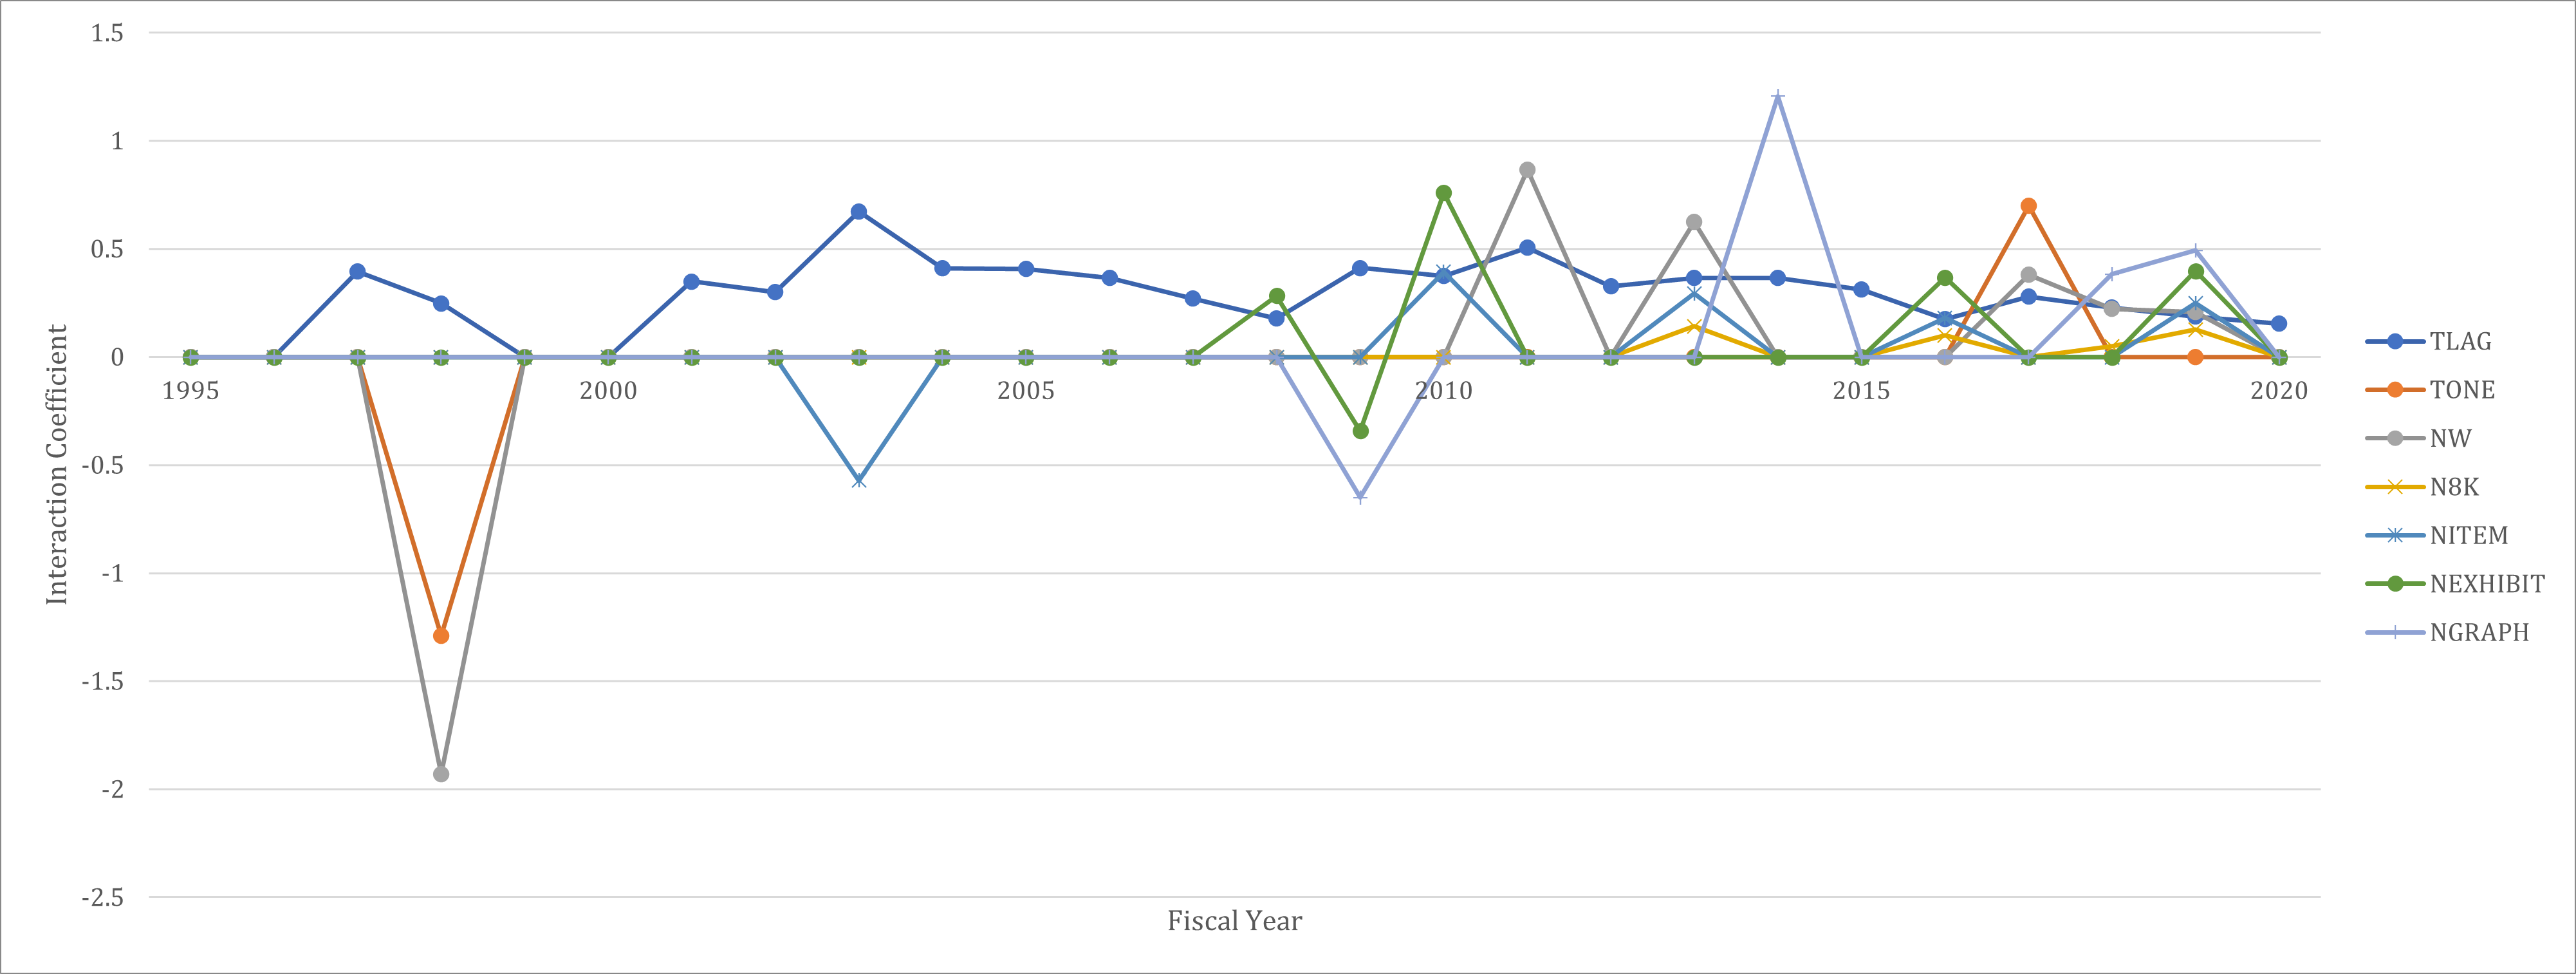
\includegraphics[scale=0.7]{../output/fig/fig2_time_trend_8K.png}
		\end{center}
	\end{figure}

\begin{footnotesize}
	\setcounter{equation}{0}
	\begin{equation}
		TEX_{i,t}=\beta_0+\beta_1\Delta DRET_{i,t-tlag}+\beta_2BN_{i,t-tlag}+\beta_3\Delta DRET_{i,t-tlag}\times 	BN_{i,t-tlag}+\sum\beta_nCONTROLS_{i,t}+\epsilon_{i,t}
	\end{equation}

	\noindent Figure 2 illustrates the time trend of narrative conservatism. X axis represents fiscal year and Y axis represents significant $\beta_3$s obtained from yearly regressions as specified by Equation \eqref{eq1}. Insignificant $\beta_3$s are replaced with zero. The coefficients of TLAG and TONE regressions are multiplied by -0.1 and 0.1 respectively to be comparable in economic magnitude to the coefficients of the rest of textual attributes.  
\end{footnotesize}
\end{landscape}